\chapter{Materiales y Métodos}
\label{ch:Instrumentacion}

Toda la información presentada en este capítulo es obtenida de los manuales de referencia del fabricante de equipos de medición Atlas Scientific, así como las imágenes de referencia presentadas también son extraídas de 
dichos manuales u hojas de datos, así como del sitio web del fabricante, https://atlas-scientific.com/.

\section{Medición de Temperatura}

%\subsection{Sonda de Temperatura PT-1000}

La \autoref{fig:figura500_1} muestra la sonda de temperatura PT-1000 utilizada para la recolección de datos de la variable de temperatura.

\begin{figure}[h]
	\centering
	\includegraphics[scale=0.5]{imgss110.png}
	\caption{Sonda PT-1000. Imagen obtenida del manual \textit{Atlas Scientific. PT-1000 Temperature Probe}}
	\label{fig:figura500_1}
\end{figure}

\clearpage

Las principales características de este instrumento se presentan en el siguiente listado:

\begin{itemize}
    \item El transductor te temperatura utilizado por esta sonda es una RTD (Resistance Temperature Detector, Detector de Temperatura Resistivo), cuyo material de fabricación es Platino de Clase A de alta pureza.
    \item Su rango de medición abarca desde los -200°C hasta los 850°C 
    \item Posee una exactitud de +/-(0.15+(0.002t)), donde t es el valor de temperatura medido.
    \item Tipo de conector BNC (Bayonet Neill-Concelman) para transmisión de la señal detectada en el medio donde se mide la temperatura.
    \item Expectativa de vida útil de 15 años.
    \item Material de caucho de silocona utilizado en la manguera que une al conector BNC con el transductor.
    \item Capacidad de sumergir por tiempo indefinido la totalidad de la sonda en agua dulce o salada.
    \item La limpieza del instrumento consiste en cepillar de forma suave la punta metálica para remover los residuos que pudiesen formarse con el paso del tiempo.  
\end{itemize}


Las aplicaciones típicas del instrumento se enlistan a continuación:

\begin{itemize}
    \item Uso estándar para análisis de laboratorio.
    \item Uso en suelo o tierra en prácticas de campo.
    \item Capacidad de sumergirse en una amplia variedad de líquidos, con excepción de aquellos que pudiesen dañar el material de la punta metálica o la manguera.
    \item Elegible para comunicación de los datos recolectados con los kits Hydroponics y Aquaponics de Atlas Scientific.
\end{itemize}

\subsection{Principio de Funcionamiento de la Sonda PT-1000}

En las operaciones de medición de temperatura, existen diversos materiales usados en los transductores especializados para este parámetro; algunos de los más utilizados son el níquel, el cobre y el platino. De estos 3 materiales
mencionados, el platino es el elegido ampliamente como estándar industrial para medición de temperatura contra otros materiales. La razón de esta elección es la relación de linealidad entre la resistencia o impedancia del 
material y la temperatura a la cual se encuentra. Es decir, por ejemplo para materiales como el níquel o el cobre, una gráfica de la relación entre la temperatura de dichos materiales y la impedanacia que presentan a dicha 
temperatura, resulta una relación matemática no lineal. En cambio, si el material elegido es el platino, la relación matématica entre impedancia del material y su temperatura resulta en una aproximación cercana a ser lineal. Para 
casos como este, resulta altamente preferible el uso de un material que tenga una relación que se aproxime a ser lineal, ya que esto simplifica los cálculos para valores de temperatura con base en los valores de impedancia que presenta
el transductor, en este caso de platino.

El nombre PT-1000 de la sonda hace referencia al elemento Platino mediante las letras PT, y el número 1000 se relaciona con el valor de resistencia de 1000 ohms medido en el material a una temperatura de 0°C. El cálculo de la 
temperatura con respecto a la resistencia presentada por el Platino tiene la forma (\ref{eq:ecuacion501})

\begin{equation}
	T(R)=\frac{3.908-\sqrt{17.59246-0.00232R}}{0.00116}
	\label{eq:ecuacion501}
\end{equation}

Como ya se ha mencionado, el valor de \textit{R} es la resistencia medida en el Platino en la sonda y \textit{T(R)} es la temperatura en función de la resistencia \textit{R}, expresada en grados Celsius.

\section{Medición de Potencial de Hidrógeno (pH)}

La \autoref{fig:figura500_2} muestra la sonda \textit{Consumer Grade} utilizada para la recolección de datos de la variable de pH.

\begin{figure}[h]
	\centering
	\includegraphics[scale=0.2]{imgss111.png}
	\caption{Sonda Consumer Grade para medición de pH. Imagen obtenida del manual \textit{Atlas Scientific. Consumer Grade pH Probe}}
	\label{fig:figura500_2}
\end{figure}

Sus principales características se enlistan a continuación:

\begin{itemize}
    \item Rango de medición de 2 a 13 en la escala estandarizada.
    \item Resolución en la medición de +/-(0.1).
    \item Precisión en la medición de +/-(0.1).
    \item Rango de temperatura de funcionamiento de 1°C a 60°C.
    \item Capacidad de soportar hasta 50PSI de presión en operación.
    \item Profundidad sumergible máxima de 35m; primeramente es necesario ampliar la longitud del cable de la sonda mediante cables externos compatibles.
    \item Tipo de conector SMA (SubMiniature Version A). Configurable para conector BNC mediante adaptadores externos.
    \item No disponible con sensor interno de temperatura.
    \item Capacidad de uso continuo durante 3 meses antes de requerir calibración.
    \item Expectativa de vida útil del sensor de 12 a 18 meses.
    \item Electrodo de referencia fabricado en plata/cloruro de plata (Ag/AgCl).
    \item Las sondas de medición de pH deben permanecer mojadas y no dejar que se seque la parte sensitiva del instrumento cuando éste no se encuentre en operación. El procedimiento estándar para mantener la sonda cuando no está 
    en funcionamiento es introducir la punta sensitiva de la sonda en el frasco con solución de almacenamiento incluida para este tipo de instrumento.
    \item Si la sonda es utilizada para medición en medios donde se estén llevando a cabo procesos químicos, procesos industriales o donde se tenga la presencia de soluciones con ácidos o bases altamente concentrados, es 
    necesario llevar a cabo la calibración del instrumento de forma más frecuente. Preferentemente, al menos 2 veces al mes o mayor número de veces si el uso del instrumento es en soluciones con alta concentración.    
\end{itemize}

Las aplicaciones típicas de la sonda de pH se enlistan a continuación:

\begin{itemize}
    \item Uso en pruebas de laboratorio.
    \item Uso en pruebas de campo.
    \item Medición de pH en diversos tipos de suelo.
    \item Medición en soluciones que contengan metales pesados.
    \item Elegible para comunicación de los datos recolectados con los kits Hydroponics y Aquaponics de Atlas Scientific.
\end{itemize}

\subsection{Principio de Funcionamiento de la Sonda de pH}

Una sonda de pH se encarga de medir el nivel de actividad de los iones (cationes) de Hidrógeno en un líquido.

La punta de la sonda contiene una membrana de cristal, la cual permite el paso de una cierta cantidad de cationes Hidrógeno al interior de la membrana, mientras los iones restantes permanecen en la solución que se está midiendo. 
La diferencia en la concentración de los cationes que están dentro de la membrana contra la concentración de los cationes que quedan fuera, genera una diferencia de potencial eléctrico el cual da origen a una pequeña corriente 
eléctrica. La magnitud de dicha corriente resulta proporcional al nivel de concentración de iones Hidrógeno en el líquido medido.

Específicamente, cuando la concentración de cationes Hidrógeno dentro de la membrana es menor a la concentración de los que quedan fuera, se tiene un valor de pH menor a 7, es decir, ácido. En el caso contrario, cuando la 
concentración de cationes es mayor dentro de la membrana, el pH tendrá un valor mayor a 7, es decir, alcalino. El último caso se presenta cuando la concentración de cationes dentro de la membrana es igual a la concentración 
fuera de ella; en este caso, el pH es de 7, es decir, neutro.

En la \autoref{fig:figura15856} se muestra una imagen de la escala estándar del parámetro pH.

\clearpage

\begin{figure}[h]
	\centering
	\includegraphics[scale=0.6]{imgss204.jpg}
	\caption{Escala estándar para magnitud de pH. Imagen obtenida de fuentes de internet}
	\label{fig:figura15856}
\end{figure}

\section{Medición de Potencial de Óxido-Reducción (ORP)}

La \autoref{fig:figura500_3} muestra la sonda \textit{Consumer Grade} utilizada para la recolección de datos de la variable de ORP.

\begin{figure}[h]
	\centering
	\includegraphics[scale=0.6]{imgss112.png}
	\caption{Sonda Consumer Grade para medición de ORP. Imagen obtenida del manual \textit{Atlas Scientific. Consumer Grade ORP Probe}}
	\label{fig:figura500_3}
\end{figure}

Sus principales características se enlistan a continuación:

\begin{itemize}
    \item Rango de medición de -1100mV a 1100mV.
    \item Exactitud de +/-(1.1mV).
    \item Rango de temperatura de operación de 1°C a 60°C.
    \item Capacidad de soportar hasta 50PSI de presión en operación.
    \item No recomendada para la medición en ácidos o bases fuertes, ni tampoco en procesos industriales. 
    \item Profundidad sumergible máxima de 35m; primeramente es necesario ampliar la longitud del cable de la sonda mediante cables externos compatibles.
    \item Tipo de conector SMA. Configurable para conector BNC mediante adaptadores externos.
    \item No disponible con sensor interno para medición de temperatura.
    \item Periodo de tiempo aproximado de 3 meses antes de requerir recalibración.
    \item Expectativa de vida útil aproximada del sensor de 12 a 18 meses.
    \item Cuando la sonda no está en uso, su almacenamiento debe ser introduciendo la punta metálica de platino en la solución para conservación incluida con el instrumento.
    \item Si el uso de la sonda es en medios donde se llevan a cabo reacciones químicas agresivas, es recomendable realizar la calibración de la sonda antes de cada uso.
    \item Si a la sonda al estar almacenda la punta metálica de platino en su solución para conservación, se le llegasen a formar residuos blancos en el tubo de cristal, dichos residuos son Cloruro de Potasio (\textit{KCl}). Antes de 
    volver a usar la sonda, enjuagarla con agua destilada hasta retirar todos los residuos. 
\end{itemize}

Las aplicaciones típicas del instrumento se enlistan a continuación:

\begin{itemize}
    \item Uso en pruebas de laboratorio.
    \item Uso en pruebas de campo.
    \item Medición en soluciones que contengan metales pesados.
    \item Elegible para comunicación de los datos recolectados con los kits Hydroponics y Aquaponics de Atlas Scientific.
\end{itemize}

\subsection{Principio de Funcionamiento de la Sonda de ORP}

Una sonda de ORP tiene como propósito medir o detectar la actividad de los electrones presentes en un líquido.

Las mediciones del parámetro de ORP representan qué tan fuerte es la transferencia de electrones a una sustancia o desde una sustancia en un líquido. Resaltando que la medición de ORP no tiene relación con la cantidad de 
electrones disponible en el líquido para una transferencia de cargas entre diferentes sustancias. Por lo tanto, expresado de otra forma, un transductor de ORP lo que hace es detectar la pequeña corriente eléctrica generada 
en el agua cuando existe un fenómeno de oxidación o reducción de otra sustancia en dicho líquido.

La sonda de ORP de Atlas Scientific está integrada por una punta metálica de platino, la cual se encuentra conectada a un conductor de plata, rodeado o inmerso en el compuesto Cloruro de Plata (AgCl). Adicionalmente, este 
conductor de plata se encuentra en contacto con una sustancia de referencia de Cloruro de Potasio (KCl). El material de platino en la punta metálica de la sonda es usado debido a que este metal se mantiene inactivo cuando se 
introduce en un líquido para realizar mediciones, es decir, dicho material se mantiene al margen de cualquier actividad electrónica que pudiése estar ocurriendo en el líquido.

\clearpage

\section{Medición de Conductividad Eléctrica}

La \autoref{fig:figura500_4} muestra la sonda \textit{K 0.1} utilizada para la recolección de datos de la variable de conductividad eléctrica.

\begin{figure}[h]
	\centering
	\includegraphics[scale=0.2]{imgss113.png}
	\caption{Sonda K 0.1 de medición de electroconductividad. Imagen obtenida del manual \textit{Atlas Scientific. Conductivity Probe K 0.1}}
	\label{fig:figura500_4}
\end{figure}

Sus principales características se enlistan a continuación:

\begin{itemize}
    \item Rango de medición de 0.07$\mu$S/cm a 50000$\mu$S/cm.
    \item Exactitud de +/-(2\%)
    \item Rango de temperatura de operación de 1°C a 110°C.
    \item Capacidad de soportar hasta 500PSI de presión en operación.
    \item Profundidad sumergible máxima de 352m; primeramente es necesario ampliar la longitud del cable de la sonda mediante cables externos compatibles.
    \item Tipo de conector SMA. Configurable para conector BNC mediante adaptadores externos.
    \item No disponible con sensor interno de temperatura.
    \item Expectativa de vida útil aproximada del sensor de 10 años.
    \item Superficie sensitiva de medición fabricada en material Grafito.
    \item Sumergible tanto en agua dulce como agua salada.
    \item La sonda K 0.1 trabaja al medir la corriente eléctrica generada en el agua entre sus 2 placas de grafito. Mientras dichas placas no se dañen ni tengan que ser reemplazadas, no es necesario realizar recalibración, 
    es decir, la primera calibración realizada antes de su primer uso es la única indispensable. 
\end{itemize}

Las aplicaciones típicas de este instrumento se enlistan a continuación:

\begin{itemize}
    \item Uso en pruebas de laboratorio.
    \item Uso en prácticas de campo.
    \item Medición en acuarios o pesceras.
    \item Elegible para comunicación de los datos recolectados con los kits Hydroponics y Aquaponics de Atlas Scientific.
    \item Medición en mezclas acuosa/orgánica.
    \item Medición en líquidos con presencia de metales pesados.
    \item Muestreo en suelos húmedos.
    \item Medición en sustancias o agentes reductores fuertes.
\end{itemize}

\subsection{Principio de Funcionamiento de la Sonda K 0.1}

La sonda K 0.1 de Atlas Scientific se encarga de realizar mediciones de la conductividad eléctrica en la solución líquida donde se sumerge. Las mediciones de conductividad en líquidos generalmente tiene como propósito el conocer 
la concentración de sales, nutrientes o impurezas.

Dentro de la sonda K 0.1, se encuentran 2 electrodos posicionados de forma opuesta uno del otro. Dada esta configuración, una vez que la sonda es sumergida en el líquido a ser analizado, un voltaje es aplicado entre dichos 
electrodos ocasionando que los cationes presentes en el líquido se desplazen hacia el electrodo polarizado con carga negativa, mientras que los aniones que se encuentren en el líquido se desplazarán hacia el electrodo que presenta
carga neta positiva. Por lo tanto, entre mayor sea la concentración de iones en el líquido analizado, mayor será la corriente generada entre los electrodos.

Es muy importante que al momento de realizar mediciones con la sonda K 0.1, el usuario continuamente verifique que no se formen burbujas entre las 2 celdas o electrodos, ya que este fenómeno afectará considerablemente los valores 
medidos. Cuando dicho fenémeno se presente, es necesario que el usuario genere sobre la sonda pequeños golpes para retirar los cúmulos de burbuja que pudieran estar presentes.

Con el paso del tiempo y el uso del instrumento, es probable que exista la formación de residuos en las áreas sensibles de la sonda, lo cual podría afectar las propiedades eléctricas de las celdas o electrodos y generar mediciones 
erróneas. Por lo cual es necesario que el usuario haga uso de un cepillo de cerdas suaves para remover dichos residuos.


\clearpage

\section{Medición de Oxígeno Disuelto}

La \autoref{fig:figura500_5} muestra la sonda \textit{Lab Grade} utilizada para la recolección de datos para el parámetro de Oxígeno Disuelto.

\begin{figure}[h]
	\centering
	\includegraphics[scale=0.6]{imgss114.png}
	\caption{Sonda Lab Grade para Oxígeno Disuelto. Imagen obtenida del manual \textit{Atlas Scientific. Lab Grade D.O. Probe}}
	\label{fig:figura500_5}
\end{figure}

Sus principales características se enlistan a continuación:

\begin{itemize}
    \item Rango de medición de 0mg/L a 100mg/L.
    \item Exactitud de +/-(0.05mg/L).
    \item Rango de temperatura de operación de 0°C a 60°C.
    \item Capacidad de soportar hasta 500PSI de presión en operación.
    \item Profundidad sumergible máxima de 352m; primeramente es necesario ampliar la longitud del cable de la sonda mediante cables externos compatibles.
    \item Tipo de conector SMA. Configurable para conector BNC mediante adaptadores externos.
    \item No disponible con sensor interno de temperatura.
    \item Periodo de tiempo aproximado de 1 año antes de requerir recalibración.
    \item Expectativa de vida útil aproximada del sensor de 4 años.
    \item Sumergible en agua dulce o salada.
\end{itemize}

\clearpage

Las aplicaciones típicas de la sonda Lab Grade son las siguientes:

\begin{itemize}
    \item Uso en pruebas de laboratorio.
    \item Uso en pruebas de campo.
    \item Uso en actividades de cuidado y preservación de especies acuáticas.
    \item Uso en producción de vino.
    \item Uso para monitoreo de condiciones ambientales.
\end{itemize}

\subsection{Principio de Funcionamiento de la Sonda Lab Grade}

La sonda Lab Grade de Atlas Scientific es una sonda galvánica para medición de Oxígeno Disuelto que consiste de una membrana de tipo PTFE (Politetrafluoroetileno), un ánodo bañado o inmerso en electrolito y su cátodo correspondiente.
Cuando la sonda es sumergida en el líquido analizado, las moléculas de oxígeno se difunden a través de la membrana; cuando ha ocurrido lo anterior, las moléculas de oxígeno son reducidas por medio del cátodo, generando una 
pequeña diferencia de potencial eléctrico. En caso de no haber moléculas de oxígeno presentes, la sonda entregará una señal eléctrica de 0V. Es decir, entre mayor sea la concentración de moléculas de oxígeno presentes, mayor 
será la señal en milivoltios entregada por el instrumento.

Importante resaltar que esta sonda galvánica en específico tiene la capacidad de entregar una señal en el rango de 0mV a 60mV, dependiendo de la saturación de oxígeno dentro de la membrana.

Con el uso continuo de la sonda, es probable que alrededor de la zona sensitiva del instrumento se formen residuos de cloruro de potasio (KCl) provenientes del electrolito del interior. Cuando esto ocurra, es necesario enjuagar 
con agua destilada la zona afectada por los residuos hasta que quede libre de ellos. Finalmente, muy importante que si los residuos se forman directamente en la zona de la membrana sensitiva, bajo ninguna circunstancia se debe 
cepillar la zona para retirarlos, ya que esto dañara la membrana y las mediciones comenzarán a ser erróneas. En este caso, es recomendable usar detergente líquido para enjuagar la zona hasta retirar los residuos acumulados.

\clearpage

\section{Equipo Wi-Fi Pool Kit de Atlas Scientific}

La \autoref{fig:figura500_6} muestra una imagen del equipo. Externamente la caja contiene en la parte frontal 4 conectores de tipo SMA, que permiten poder conectar 4 sondas de medición, dando de esta forma la posibilidad de medir el mismo tiempo 4 parámetros en la muestra de agua 
analizada. En la parte trasera, se tiene un conector USB Tipo B para la alimentación y comunicación por medio de una computadora externa. Internamente contiene 4 circuitos de instrumentación para acondicionamiento de las señales entregadas por las sondas en uso. Estas 4 tarjetas PCB envían los datos previamente procesados a un microcontrolador ESP32.

\begin{figure}[h]
	\centering
	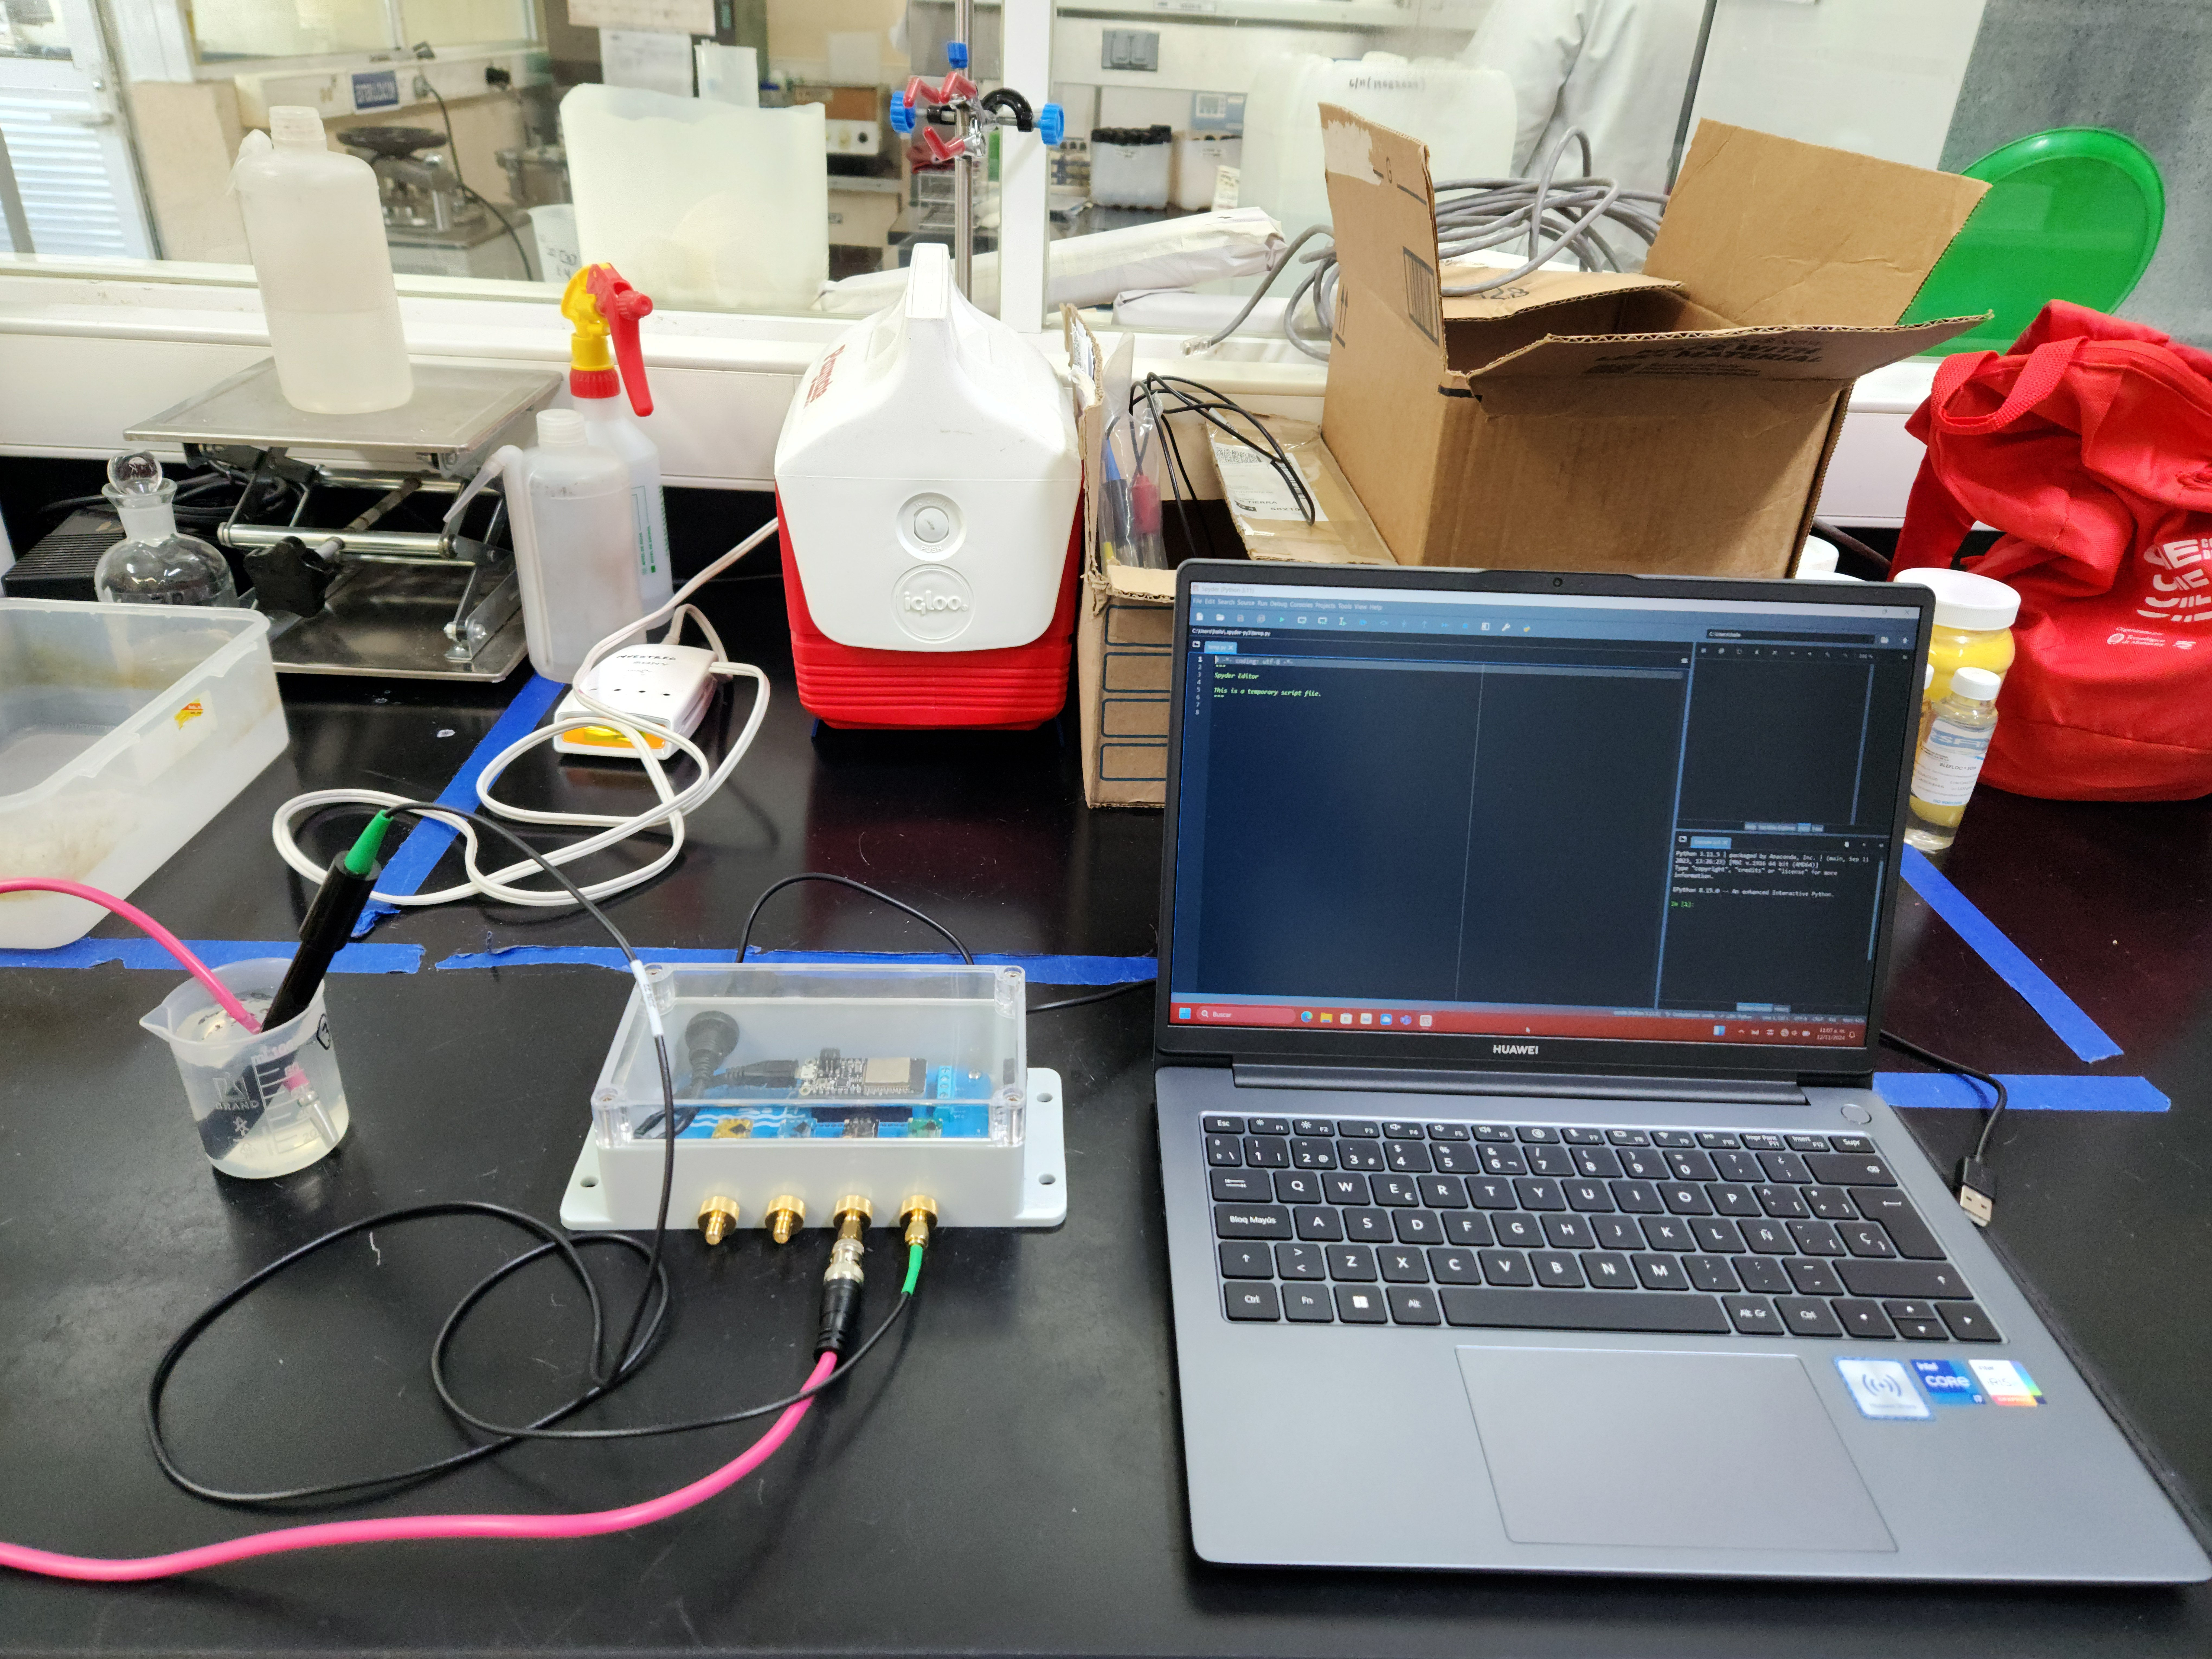
\includegraphics[scale=0.05]{imgss203.jpg}
	\caption{Wi-Fi Pool Kit.}
	\label{fig:figura500_6}
\end{figure}

La metodología utilizada para trabajar con este equipo consiste primeramente en la recolección de las muestras de agua que serán caracterizadas. Una vez que las muestras se tienen disponibles en frascos de muestreo, se sumergen 
en ella 4 sondas de los parámetros deseados, las cuales también son conectadas a los puertos SMA. Una vez que se tiene dicha configuración, el kit debe conectarse a una computadora para iniciar la comunicación con el 
microcontrolador ESP32, el cual está recibiendo secuencialmente un registro de 4 datos correspondiente a las 4 sondas utilizadas. Este registro de 4 valores numéricos es posible imprimirlos en la terminal del IDE de Arduino,
para posteriormente exportar dichos registros a un archivo CSV. externo donde quedarán almacenados todos los registros recolectados, para su posterior uso para análisis de estadística descriptiva y tareas de entrenamiento y 
validación en modelos clasificadores para estimación de Calidad del Agua.

Las principales prestaciones del kit Wi-Fi Pool se detallan a continuación.

\begin{itemize}
    \item El equipo viene configurado de fabrica para realizar la medición de los parámetros de temperatura, pH y ORP; el cuarto puerto disponible auxiliar está disponible para la conexión de otro circuito de acondicionamiento 
    de señal para el monitoreo del cuarto y último parámetro disponible para este equipo.
    \item El equipo está diseñado para que el usuario pueda modificar sus funcionalidades. Es decir, el usuario puede cambiar tarjetas de acondicionamiento de señal disponibles por otras diferentes para otros parámetros adicionales,
    de acuerdo a las necesidades que se tengan.
    \item Equipo controlado mediante un microcontrolador ESP32, programable mediante la plataforma Arduino IDE.
    \item Los puertos de pH, ORP y el Auxiliar tienen aislamiento eléctrico; el puerto destinado para temperatura no dispone de dicha característica.
    \item El circuito requiere alimentación de 5V de CC en caso de no tener disponibilidad de conexión con una computadora, y se requiera alimentar mediante un adaptador o regulador externo.
    \item El microcontrolador ESP32 utiliza el protocolo I2C para comunicación con las tarjetas de acondicionamiento de señal. No es posible configurarlo para comunicación mediante protocolo UART en caso de ser 
    requerido por el usuario.
    \item Si el usuario requiere conectar diferentes tarjetas de acondicionamiento de señal a las ya incluidas, es necesario primero asegurarse que dichos circuitos previamente estén configurados para comunicación mediante 
    protocolo I2C.
    \item La interfaz de Arduino IDE permite la calibración de los circuitos de acondicionamiento de señal mediante el uso de comandos específicos desde la terminal del IDE.
\end{itemize}

\section{Calibración de los Sondas de Medición}

\subsection{Sonda de Temperatura}

Para realizar la calibración de la sonda de temperatura PT-1000 primeramente es necesario tener disponible un recipiente con agua hirviendo, la cual en teoría se encuentra a una temperatura de 100°C, sin embargo, el punto 
de ebullición del agua varía conforme la altura; a nivel del mar el punto de ebullición es de 100°C, y conforme la altura sobre el nivel del mar aumenta, el punto del ebullición del agua decrece un pequeño porcentaje.

Una vez que ya se tiene disponible el agua en su punto de ebullición, se debe conectar la sonda de temperatura al equipo Pool Kit en el conector correspondiente, y cargar al microcontrolador el código fuente disponible para 
descarga desde el sitio web de Atlas Scientific. Una vez que ya se tiene la conexión descrita, la punta de la sonda debe sumergirse en el agua hirviendo y posteriormente en la terminal del Arduino IDE, por comunicación serial, ejecutar el comando 
\textbf{rtd:cal,t}

\subsection{Sonda de pH}

Para la calibración de la sonda de pH se requiere de 3 soluciones de calibración específicas, para valor medio o neutro, valor bajo y valor alto. La solución de calibración de valor bajo contiene un compuesto a un pH de 
valor de 4, la solución de valor medio o neutro contiene un compuesto a un valor 7 de pH y la solución de valor alto contiene líquido de calibración a un valor 10 de pH.

Primeramente se debe tener conectada la sonda de pH al equipo Pool Kit en el conector correspondiente y el microcontrolador del equipo debe ejecutar el código fuente del fabricante Atlas Scientific. Una vez que se tiene 
listo lo descrito anteriormente, la sonda de pH debe introducirse en la solución de valor 7 de pH y esperar un rango de tiempo de 1 a 2 minutos mientras se estabilizan los valores medidos mostrados en la terminal del Arduino
IDE. Una vez que las lecturas mostradas en la terminal son estables, en terminal se debe ejecutar el comando \textbf{ph:cal,mid,7}; una vez terminado lo anterior, se tiene la sonda calibrada para valores neutros y la solución 
de calibración de valor 7 de pH debe desecharse ya que después de varios minutos de abierto el empaque, el líquido pierde sus propiedades. 

Finalmente, el proceso anterior debe repetirse para las soluciones de valor 4 y 10 de pH, las cuales requerirán los comandos \textbf{ph:cal,low,4} y \textbf{ph:cal,high,10}, respectivamente.

\subsection{Sonda de ORP}

El procedimiento para la calibración de la sonda de ORP consiste en el uso de la solución de calibración que proporciona el fabricante Atlas Scientific junto con el equipo Pool Kit. Primeramente es necesario tener la sonda 
de ORP conectada al equipo en su conector correspondiente y el microcontrolador ejecutando el código fuente desarrollado por el fabricante para este kit específico. Una vez que se tiene el equipo y la sonda en funcionamiento,
es necesario introducir la sonda dentro de la solución de calibración, la cual está diseñada para proveer un ORP con valor de 225mV. Una vez que se han estabilizado las lecturas impresas en la terminal del Arduino IDE, es 
necesario ejecutar el comando \textbf{orp:cal,225} con el cual el circuito quedará calibrado teniendo como referencia este valor dado por esta solución específica.

En caso de que el usuario tenga a su disposición una solución de calibración diferente a la del fabricante Atlas Scientific, es posible usar dicha solución si es que se conoce el valor de referencia nominal para dicha solución,
además de ser recomendable tener la tabla de valores para dicho compuesto de la variación del ORP con la temperatura. Es decir, dicha solución de calibración externa tendrá un valor nominal original de ORP, 
sin embargo, el valor de temperatura a la que se encuentre generará variaciones en su valor de ORP y poseer la tabla de referencia servirá para conocer el valor exacto de ORP según la temperatura a la cual se encuentre. 

En caso de que el usuario decida usar una solución de calibración diferente a la de Atlas Scientific, el comando de calibración a ejecutar en la terminal viene siendo \textbf{orp:cal,valor}; en dicho comando el factor 
\textbf{valor} viene siendo el valor de ORP dado para la solución de calibración que se esté manejando.

\subsection{Sonda de Conductividad Eléctrica}

La sonda de electroconductividad es de calibración única, es decir, antes de usarse por primera vez se realiza la calibración y posteriormente no es necesario volver a realizarla, aunque si después de cierto tiempo de uso 
el usuario desea volver a realizar la calibración, se puede ejecutar sin ningún problema.

Para realizar la calibración de esta sonda es necesario tenerla conectada al equipo Pool Kit en su conector correspondiente y el microcontrolador se encuentre ejecutando el código fuente dado por el fabricante. Dado lo anterior,
primeramente se debe realizar la calibración en seco, para la cual se debe tener la sonda al aire libre y ejecutar el comando \textbf{ec:cal,dry}. Una vez que la calibración en seco ha finalizado, el siguiente paso es realizar 
la calibración para un valor bajo usando la solución proporcionada por el fabricante Atlas Scientific; la sonda debe introducirse en la solución dada y esperar a que se estabilicen las mediciones mostradas en la terminal del IDE,
para poder ejecutar el comando \textbf{ec:cal,low,12880}. 

Una vez realizada la calibración para un valor bajo de referencia, se debe realizar la calibración para un valor alto; al finalizar la calibración para valor bajo, es necesario enjuagar completamente la sonda para eliminar 
residuos de la solución de valor bajo, y posteriormente poder introducirla en la solución de valor alto de referencia. Una vez que han estabilizado las mediciones mostradas en la terminal del IDE para la solución de valor 
alto, se debe ejecutar el comando \textbf{ec:cal,high,80000} y el proceso de calibración estará completo.

\subsection{Sonda de Oxígeno Disuelto}

Para la calibración de la sonda de oxígeno disuelto primeramente es necesario tener la sonda conectada al equipo Pool Kit y su microcontrolador ejecutando el código fuente dado por el fabricante. Posteriormente, es necesario 
dejar la sonda expuesta al aire libre por lo menos 30 segundos o hasta que las lecturas impresas en la terminal del Arduino IDE sean estables. Una vez que los valores medidos se han estabilizado, es necesario ejecutar en 
la terminal el comando \textbf{do:cal}, con lo cual la calibración estará completa.

Inmediatamente después que la calibración se ha llevado a cabo, en la terminal del IDE Arduino los datos medidos de oxígeno disuelto deben estar en el rango de 9.09mg/L a 9.2mg/L aproximadamente; estos valores pueden variar 
según sea la temperatura, salinidad y presión atmosférica a la que se encuentre el equipo.

\section{Configuración de la tarjeta PCB del equipo WiFi Pool Kit de Atlas Scientific}

La \autoref{fig:figura500_7} muestra un esquema de la placa donde se montan los componentes para acondicionamiento de señal y el microcontrolador ESP32 para comunicación con una computadora externa.

\begin{figure}[h]
	\centering
	\includegraphics[scale=0.9]{imgss207.png}
	\caption{Esquema de la conexión en PCB. Imagen obtenida del manual \textit{Wi-Fi Pool Kit Setup Guide}}
	\label{fig:figura500_7}
\end{figure}

En la parte inferior de la \autoref{fig:figura500_7} se observan los conectores para las 4 sondas disponibles para lectura de datos, teniendo originalmente conexiones para las variables de temperatura, pH, y ORP; se cuenta 
en la conexión más a la derecha una cuarta opción adicional, pero el circuito de instrumentación debe ser elegido por el usuario según la variable que se requiera monitorear.

En la parte central se encuentran los espacios disponibles para las tarjetas PCB que ya montan circuitos para acondicionamiento de las señales eléctricas medidas por las sondas, para posteriormente transmitir al microcontrolador 
los valores de variables convertidos a su escala correspondiente. 

La \autoref{fig:figura500_8} muestra una imagen para el circuito de acondicionamiento del parámetro de temperatura.

\begin{figure}[h]
	\centering
	\includegraphics[scale=0.7]{imgss208.png}
	\caption{EZO RTD Temperature Circuit. Imagen obtenida del sitio \textit{https://atlas-scientific.com/}}
	\label{fig:figura500_8}
\end{figure}

Para este circuito el pin \textit{VCC} debe conectarse a una alimentación de 5V, el pin \textit{GND} requiere conexión a una tierra de referencia, y los pines \textit{TX} y \textit{RX} son las conexiones para transmisión y 
recepción de datos, respectivamente; estos pines llevan a los pines de comunicación correspondientes del ESP32. El protocolo de comunicación para esta tarjeta puede ser \textit{UART} o \textit{I2C}, sin embargo, para el ESP32 
se requiere exclusivamente usar \textit{I2C} como protocolo.

Otras características de esta tarjeta son las siguientes:

\begin{itemize}
    \item Resolución de 0.001 para las operaciones matemáticas de conversión de voltaje a salida de dato de temperatura.
    \item Capacidad para realizar máximo 1 lectura por segundo.
    \item Empleo del formato ASCII para la comunicación serial.
    \item Rango de voltaje de operación de 3.3V-5.5V.
\end{itemize}

La \autoref{fig:figura500_9} muestra una imagen para el circuito de acondicionamiento del parámetro de pH.

\clearpage

\begin{figure}[h]
	\centering
	\includegraphics[scale=0.7]{imgss209.png}
	\caption{EZO pH Circuit. Imagen obtenida del sitio \textit{https://atlas-scientific.com/}}
	\label{fig:figura500_9}
\end{figure}

En esta tarjeta el pin \textit{VCC} debe conectarse a una alimentación de 5V, el pin \textit{GND} requiere conexión a una tierra de referencia, y los pines \textit{TX} y \textit{RX} son las conexiones para transmisión y 
recepción de datos, respectivamente; estos pines llevan a los pines de comunicación correspondientes del ESP32. El protocolo de comunicación para esta tarjeta puede ser \textit{UART} o \textit{I2C}, sin embargo, la comunicación 
serial con la tarjeta ESP32 requiere exclusivamente \textit{I2C} como protocolo.

Otras características de esta tarjeta son las siguientes:

\begin{itemize}
    \item Rango de medición en escala estándar de ph desde 0.001 hasta 14.000.
    \item Resolución de 0.001 para la conversión de voltaje a dato pH de salida.
    \item Tiempo de 800ms necesario para ejecutar una lectura.
    \item Capacidad de recibir señales de entrada de cualquier tipo de sonda especializada para el parámetro de pH.
    \item Capacidad para comunicación serial mediante \textit{I2C} o \textit{UART} como protocolos.
    \item Formato ASCII en la comunicación serial.
\end{itemize}

La \autoref{fig:figura500_10} muestra una imagen para el circuito de acondicionamiento del parámetro de ORP.

\clearpage

\begin{figure}[h]
	\centering
	\includegraphics[scale=0.7]{imgss210.png}
	\caption{EZO ORP Circuit. Imagen obtenida del sitio \textit{https://atlas-scientific.com/}}
	\label{fig:figura500_10}
\end{figure}

Para esta tarjeta las conexiones de los pines son las mismas que las mencionadas para los casos anteriores, es decir, se requiere la alimentación de 5V, un punto de referencia a tierra y los pines de comunicación para la 
transmisión y recepción de datos con el dispositivo ESP32.

Las características principales para este circuito son las siguientes:

\begin{itemize}
    \item Rango de medición de voltaje de entrada desde -1.2V hasta 1.2V.
    \item Precisión de +/-1mV.
    \item Capacidad máxima de lectura de 1 dato por segundo.
    \item Compatibilidad para recibir señales de entrada de cualquier tipo de sonda para ORP.
    \item Comunicación serial UART o I2C mediante codificación ASCII.
    \item Su calibración se puede realizar para cualquier valor de ORP conocido.
\end{itemize}

La \autoref{fig:figura500_11} muestra una imagen para el circuito de acondicionamiento del parámetro de conductividad.

\clearpage

\begin{figure}[h]
	\centering
	\includegraphics[scale=0.7]{imgss211.png}
	\caption{EZO Conductivity Circuit. Imagen obtenida del sitio \textit{https://atlas-scientific.com/}}
	\label{fig:figura500_11}
\end{figure}

Para este circuito se requiere alimentación de 5V en el pin \textit{VCC}, referencia de tierra para la conexión \textit{GND} y las conexiones para comunicación serial con el microcontrolador ESP32 en los pines \textit{TX} 
y \textit{RX}.

Las propiedades para esta tarjeta son las siguientes:

\begin{itemize}
    \item Capacidad para lecturas de los parámetros de conductividad, sólidos disueltos totales, salinidad y gravedad específica exclusivamente en agua de mar.
    \item Tiempo de 600ms requerido para ejecutar una lectura.
    \item Lecturas de 4 dígitos para valores de conductividad mayores o iguales a 10$\mu$S/cm.
    \item Lecturas de 3 dígitos para valores de conductividad igual o menores a 9.99$\mu$S/cm. 
\end{itemize}

Finalmente, la \autoref{fig:figura500_12} muestra el circuito para lecturas de la variable de oxígeno disuelto.

\clearpage

\begin{figure}[h]
	\centering
	\includegraphics[scale=0.7]{imgss212.png}
	\caption{EZO Dissolved Oxygen Circuit. Imagen obtenida del sitio \textit{https://atlas-scientific.com/}}
	\label{fig:figura500_12}
\end{figure}

Los pines de conexión para esta placa requieren las mismas condiciones que los casos anteriores. Sus características principales son las siguientes:

\begin{itemize}
    \item Rango de lecturas de salida desde 0mg/L hasta 100mg/L. 
    \item Precisión de +/-0.05mg/L.
    \item Tiempo de 600ms requerido para la ejecución de cada lectura individual.
    \item Compatibilidad para lectura de voltajes de entrada exclusivamente de sondas de tipo galvánicas.
    \item Compensación para variaciones de temperatura, salinidad y presión atmosférica.
\end{itemize}

En lo referente a las conexiones de los circuitos de acondicionamiento de señal con el microcontrolador, en la \autoref{fig:figura500_13} se muestra un circuito esquemático de la conexión completa para el equipo Pool Kit.

\clearpage

\begin{figure}[h]
	\centering
	\includegraphics[scale=0.7]{imgss213.png}
	\caption{Diseño esquemático del PCB para el equipo Pool Kit. Imagen obtenida del manual \textit{Wi-Fi Pool Kit Setup Guide}}
	\label{fig:figura500_13}
\end{figure}

Para este diseño, los circuitos de ORP, pH y el AUX (circuito auxiliar) incluyen aislamiento electrico; el circuito de temperatura no contempla el aislamiento debido a que el elemento sensitivo en la sonda de temperatura 
no entra en contacto directo con el agua. Para esta implementación en específico la alimentación de todo el circuito se realiza a través del microcontrolador, así como también el punto de tierra de referencia se toma de 
la tarjeta del microcontrolador.

Es importante resaltar que esta implementación permite al usuario reemplazar los circuitos de acondicionamiento por otros para parámetros de calidad del agua diferentes. El único requisito es que los nuevos circuitos deben 
previamente estar diseñados o configurados para comunicación con I2C como protocolo, ya que en este caso el microcontrolador no esta adaptado para comunicación serial UART.

\section{Conclusiones}

En este capítulo se describen las posibilidades de generar equipo de medición para variables de calidad del agua al combinar sensores con el diseño de un sistema embebido compuesto de microcontrolador y tarjetas PCB con 
circuitos de instrumentación para acondicionamiento de las señales dadas por los sensores.

Es relevante cómo un número importante de parámetros de calidad del agua pueden ser monitoreados con este tipo de diseños, únicamente teniendo que cumplir los requerimientos de diseño específicos para cada circuito de 
instrumentación, atendiendo a las características individuales de cada señal eléctrica generada en los sensores para cada variable distinta.
